% Created 2023-01-31 Tue 19:12
% Intended LaTeX compiler: lualatex
\documentclass[11pt]{article}
\usepackage{graphicx}
\usepackage{longtable}
\usepackage{wrapfig}
\usepackage{rotating}
\usepackage[normalem]{ulem}
\usepackage{amsmath}
\usepackage{amssymb}
\usepackage{capt-of}
\usepackage{hyperref}
\usepackage{minted}
\usepackage{physics}
\usepackage[margin=0.5in]{geometry}
\usepackage{minted}
\author{David Lewis}
\date{1/31/2023}
\title{Lec 7: Classroom activity}
\hypersetup{
 pdfauthor={David Lewis},
 pdftitle={Lec 7: Classroom activity},
 pdfkeywords={},
 pdfsubject={},
 pdfcreator={Emacs 28.2 (Org mode 9.6)}, 
 pdflang={English}}
\begin{document}

\maketitle
\section*{1.}
\label{sec:orgf8b63a5}
\begin{itemize}
\item \(S_B = (\mu_1-\mu_2)(\mu_1-\mu_2)^T\)
\item \(\mu_1 = \begin{bmatrix} 2 \\ 0 \end{bmatrix}, \mu_2 = \begin{bmatrix} 4 \\ 0 \end{bmatrix}\)
\item \(\mu_1-\mu_2 = \begin{bmatrix}-2 \\ 0 \end{bmatrix}\)
\item \(S_B = \begin{bmatrix}-2 \\ 0 \end{bmatrix} \begin{bmatrix}-2 & 0 \end{bmatrix}
  = \begin{bmatrix} 4 & 0 \\ 0 & 0 \end{bmatrix}\)
\item \(S_w = S_1 + S_2\)
\item \(S_1 = n_1 \Sigma_1 = (x-\mu)(x- \mu)^T = \begin{bmatrix} 0 & 0 \\ 0 & 8 \end{bmatrix}\)
\item \(S_2 = n_1 \Sigma_1 = (x-\mu)(x- \mu)^T = \begin{bmatrix} 0 & 0 \\ 0 & 32 \end{bmatrix}\)
\item \(S_w = \begin{bmatrix} 0 & 0 \\ 0 & 40 \end{bmatrix}\)
\item \(|S_w| = 0\) so \(S_w\) is singular
\end{itemize}
\section*{2.}
\label{sec:orgff7f154}
\begin{itemize}
\item LDA is only successful in A, not B or C
\item A is not the same as the PCA, it would be diagonal
\item B is not the same as the PCA, it would be vertical
\item C is the same as the PCA
\end{itemize}
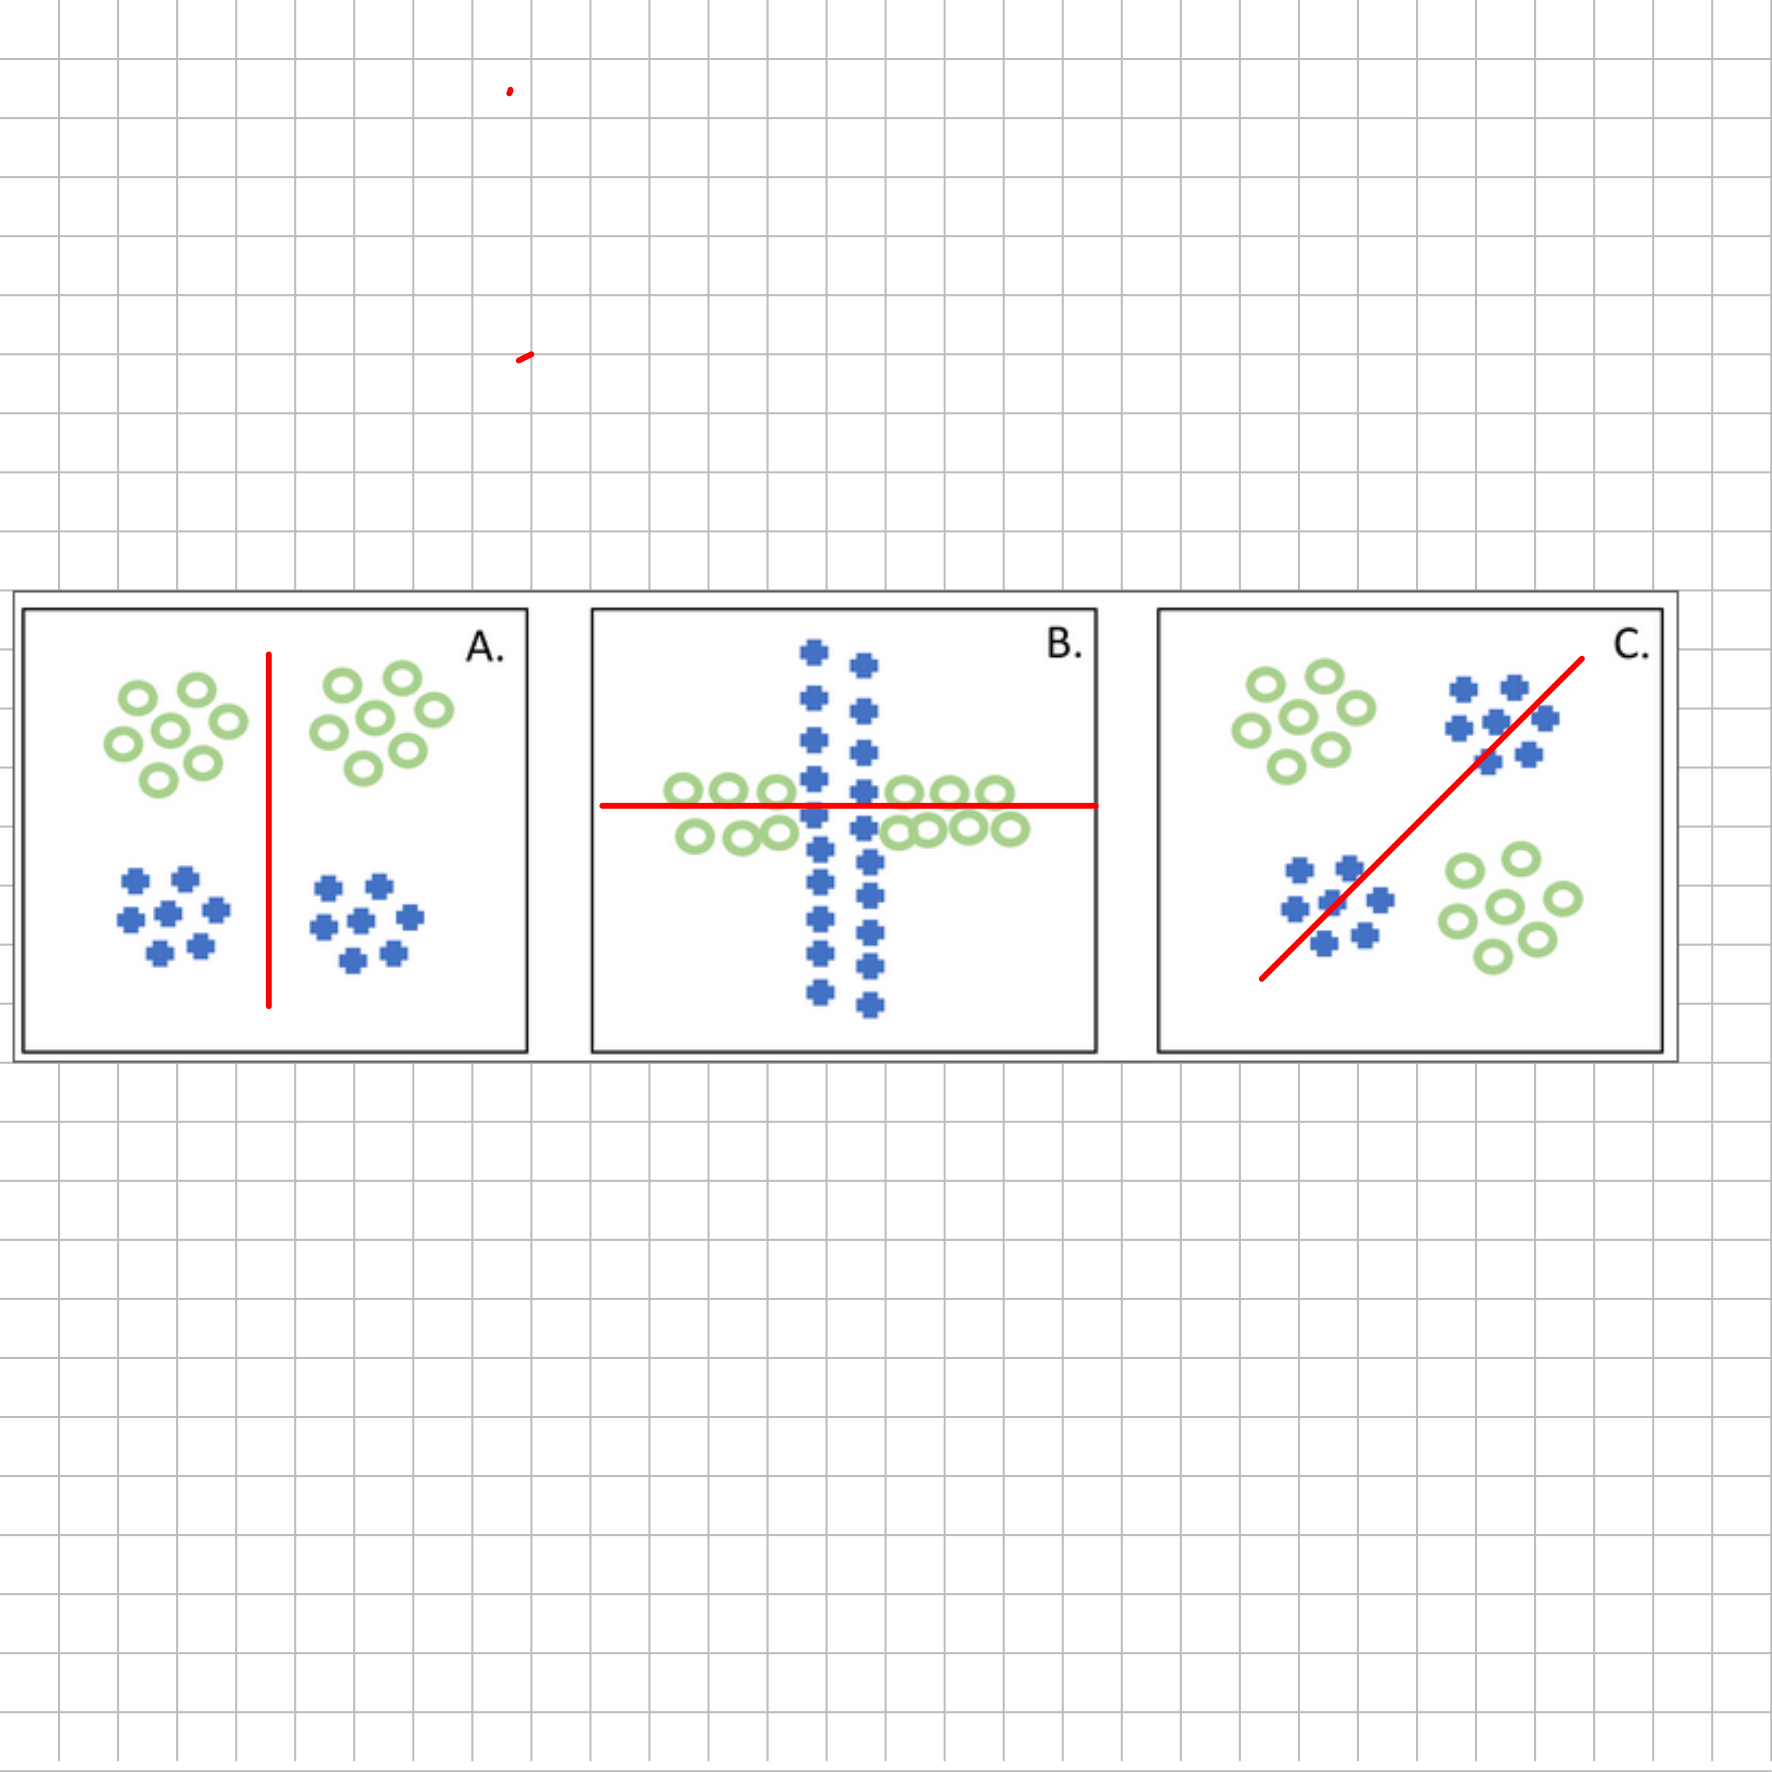
\includegraphics[width=\textheight,height=\textwidth,keepaspectratio]{/home/david/Documents/Planner/Intelligent_Data_Design/Assignments/lec7/images/lda.png}
\section*{3.}
\label{sec:org35823d3}
\begin{itemize}
\item the separation can be done with multiple curves. THis is best suited to B and C.
\end{itemize}
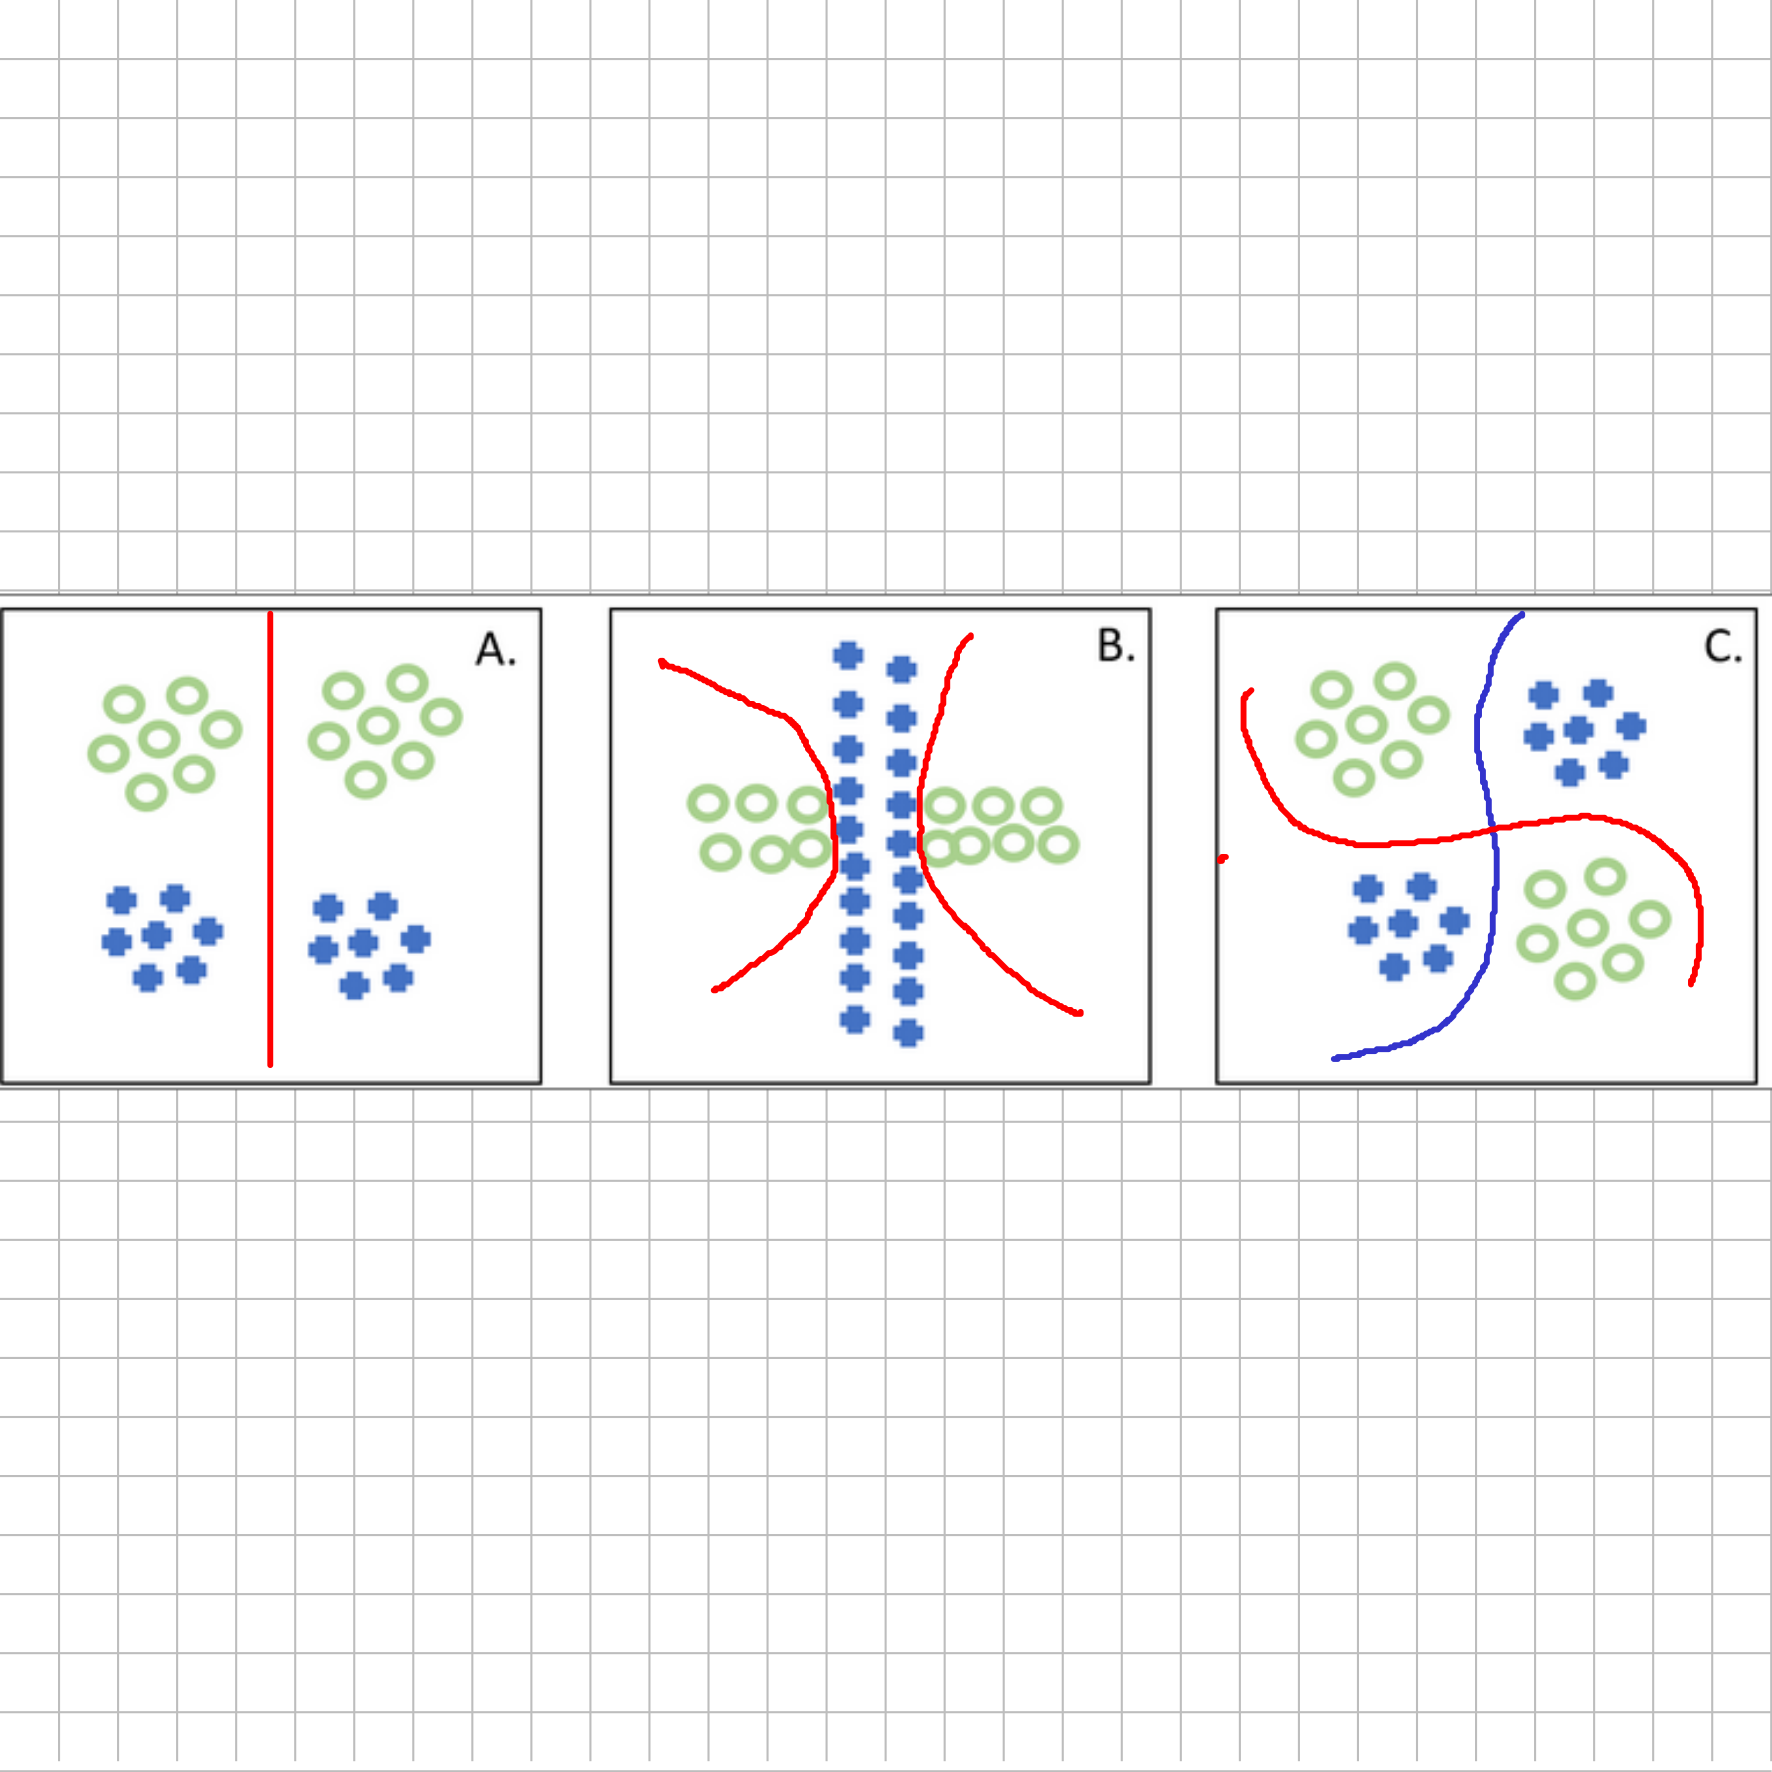
\includegraphics[width=\textheight,height=\textwidth,keepaspectratio]{/home/david/Documents/Planner/Intelligent_Data_Design/Assignments/lec7/images/lda2.png}
\section*{4.}
\label{sec:org65e11cc}
\begin{itemize}
\item \(X_{n\times d}, Y_{n\times 1}\)
\item \(x_i\) is a row vector of \(X_{n\times d}\)
\item \(y_i\) is an element of \(Y_{n\times1}\)
\item \(D_i \leftarrow \{x_j | y_i, j=1, ..., n\}, i = 1,2\)
\item \(\mu_i \leftarrow \text{mean}(D_i), i = 1,2\) =calculate the mean for
\item \(S_B \leftarrow \(\mu_1-\mu_2)(\mu_1-\mu_2)^T\) \texttt{Calculate between class matrix by multiplying the two mean vectors}
\item \(Z_i \leftarrow D_i-\mu_i^T, i = 1,2\) \texttt{Subtract the mean from matrix}
\item \(S_i \leftarrow Z^T_iZ_i, i= 1,2\) \texttt{S matrix is n * covariance matrix for each class}
\item \(S_w \leftarrow S_1 + S_2\) \texttt{Calculate Sw by summing the two S matricies}
\item \(\lambda_1,w \leftarrow eigen(S^{-1}B)\) \texttt{get dominant eigenvector,eigenvalue using the eigen function in the previous homework}
\end{itemize}
\section*{5.}
\label{sec:orgb2254b8}
\begin{itemize}
\item \(K(w) = \frac{w^TS_Ww}{w^TS_Bw}\)
\item \(\frac{d}{dx}\left(\frac{f(x)}{g(x)}\right) = \frac{f'(x)g(x) -
  g'(x)f(x)}{g(x)^2}\) definition of derivative for multiple functions
\item \(\frac{d}{dw}K(w) = \frac{2S_ww(w^TS_Bw) -  2S_Bw(w^TS_Sw)}{(w^TS_Bw)^2} =
  0\) set derivative equal to 0 to minimize the function.
\item \(2S_ww(w^TS_Bw) = 2S_Bw(w^TS_Sw)\) simplyifing
\item \(S_ww = S_Bw\frac{(w^TS_Sw)}{(w^TS_Bw)} = S_BwK(w) = \lambda S_Bw\) Substituting in
K(w), which is by definition an eigenvalue of \(S_B\) and \(S_w\).
\item If \(S_B^{-1}\) exists (nonsingular), then \(S_B^{-1}S_ww = \lambda S_B^{-1}S_Bw =
  \lambda w\) This changes the form to be the regular eigenvector eigenvalue equation.
\item \(S_B^{-1}S_ww = \lambda w\) this is the regular eigenvector eigenvalue equation,
solvable using the LDA algorithm
\end{itemize}
\end{document}
